% Multiple Choice Question 6
\begin{questions}\setcounter{question}{5}\question
A positron (charge $+e$, mass $m_{e}$) moves in a circular path of radius $R$ due to a uniform magnetic field of strength $B$ applied perpendicular to the plane of the circle. If $B$ is varied, which of the following best represents a graph of the kinetic energy of the positron as a function of $B$ so that the positron maintains the same radius $R$ ?

\begin{oneparchoices}
\choice \adjustbox{valign=t}{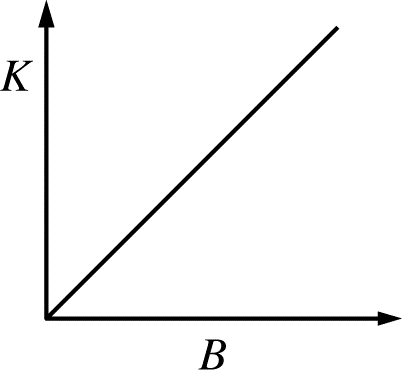
\includegraphics[scale=0.3]{images/img-005-015.png}}
\choice \adjustbox{valign=t}{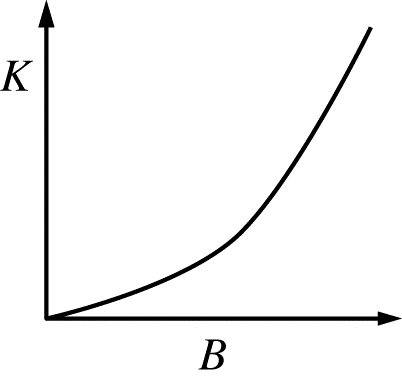
\includegraphics[scale=0.3]{images/img-005-016.png}}
\choice \adjustbox{valign=t}{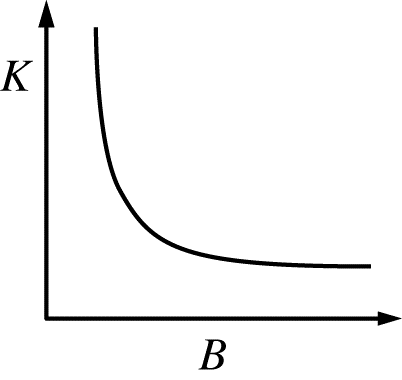
\includegraphics[scale=0.3]{images/img-005-017.png}}
\choice \adjustbox{valign=t}{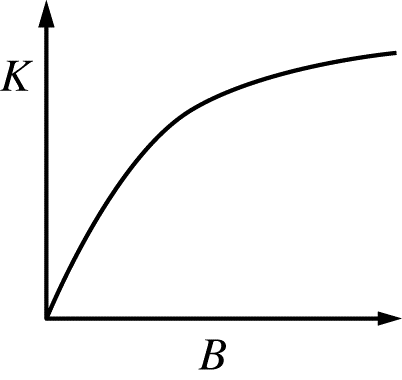
\includegraphics[scale=0.3]{images/img-005-018.png}}
\choice \adjustbox{valign=t}{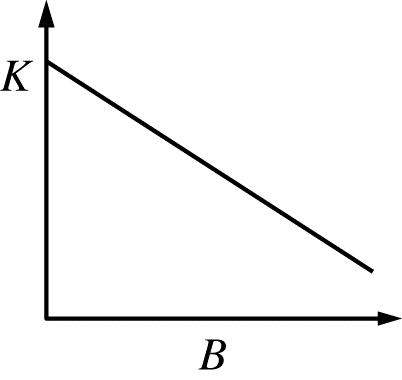
\includegraphics[scale=0.3]{images/img-005-019.png}}
\end{oneparchoices}\end{questions}

